\subsection{
  Replies to comments received from Anselmo Cervera - Jan. 08, 2013 }

\begin{enumerate}

%........................................................................................................
\vspace{5 mm}
\item
{\em
  ``At lines 545-548 you say that there are small differences in the number of events between the two productions. 
    Is this due to the different random seeds in SKDETSIM? 
    Could you be a bit more explicit and also mention that the implications are negligible.''
}\\
\\
The following two paragraphs,
explaining the changes in the second production,
 are copied verbatim from an e-mail communication with Patrick de Perio:\\
\\
`Unfortunately, the files were generated after a major cluster upgrade
which didn't support g77 anymore. Therefore, the development branch had
to be used. They are mostly equivalent to the official release, aside
from fixes to array bounds errors, for example. The major change was for
SKDETSIM: adding the new truth information necessary for reweighting.'

`There are some small differences between the official production and
this production that are not yet understood, thus this production has
not been made official and only used to evaluate the FSI+SI systematic
error. For nue, this was done by comparing the reweighted to nominal
within this sample to calculate the covariance matrix, which was then
applied to the official distributions.'\\
\\
The second production was used to evaluate uncertainties due to FSI+SI by all three 
$\nu_{e}$-appearance analyses, and these analyses were approved by the collaboration. 
It was also used by the KIT $\nu_{\mu}$-disappearance analysis. 

%........................................................................................................
\vspace{5 mm}
\item
{\em
  ``In Table 4 the page number appears on top of the caption. Can you remove the page number?''
}\\
\\
Done.

%........................................................................................................
\vspace{5 mm}
\item
{\em
  ``In Table 9, where do Total (banff prefit and postfit) come from? 
    Is the sum in quadrature of the figures above ? If this is the case I get different numbers. 
    I guess correlations are taken into account in the sum and thus the result is smaller. 
    Could you please clarify that in the text or in the caption.''
}\\
\\
The numbers were generated using an ensemble of 20,000 toy-MC experiments.
Separate runs were used for the total error and the various error components.
The statistical error using 20,000 toy-MC experiments is not negligible and this is
the cause of the difference you are observing. Table 9, will be revised
in version 2 of T2K-TN-141. 
We will increase the number of toy-MC experiments to 100,000.
The same ensemble will be used for the total error and the error components
to avoid inconsistencies between the numbers due to statistical fluctations.
The error envelopes shown in Figs. 18-22 will also be updated using the larger toy-MC ensemble.

%........................................................................................................
\vspace{5 mm}
\item
{\em
  ``I think you should specify where the fixed oscillation parameters come from (line 601-602).''
}\\
\\
Done. See also the reply to Neil's comment \#1.

%........................................................................................................
\vspace{5 mm}
\item
{\em
  ``As Neil pointed out constraining the systematic parameters within 1 $\sigma$ should be 
  justified (lines 629-630).''
}\\
\\
There was a typing mistake in the note.
See the reply to Neil's comment \#4.

%........................................................................................................
\vspace{5 mm}
\item
{\em
  ``Is is correct to exclude systematic variations leading to a negative number of predicted events.''
}\\
\\
This was discussed a number of times in the oscillation analysis group and it was decided that
this method will be adopted by all analyses, including the VaLOR and KIT $\nu_{\mu}$-disappearance analyses.
We believe this is a reasonable choice.
We chose to intrepret our data in a framework where all probabilities are well-defined.
The motivation for excluding systematic variations leading to negative numbers of events is
the same as the motivation for constraining $\sin^{2}(2\theta_{23})$ to be in the physically-allowed region.
%........................................................................................................
\vspace{5 mm}
\item
{\em
  ``Missing dot in line 630.''
}\\
\\
Fixed.

%........................................................................................................
\vspace{5 mm}
\item
{\em
  ``What is the initial value for the oscillation parameters? 
    Although the fit is repeated taking random values of those parameters is the first trial 
    also performed with random initial parameters. If so, it should be clarified. Lines 643-645''
}\\
\\
For toy-MC experiment fits where the input is known (e.g. pull studies, sensitivity studies,
calculation of Feldman and Cousins ${\Delta}\chi^{2}_{critical}$ values)
both $\sin^{2}(2\theta_{23})$ and $|\Delta m^2_{32}|$ are initialized at their true values.
All nuisance parameters included in the fit are initialized to their nominal values, except from the 
spectral function one, $f_{SF}$, which is initialized to 0.5 (away from the limits of its allowed region at 0 and 1). 

For fits to the actual data, the $\chi^2$ surface is constructed via a series of `0+N' (`0+8') fits,
as described in Sec.\ 4.5, and the grid point where the minimum $\chi^2$ occurs is found.
100 fits are performed, each initialised with random values drawn uniformly from an oscillation parameter
range $\pm$3 bins (respecting boundaries) around the grid point with the minimum $\chi^2$ value.
For each fit, random initial values are selected for all systematic parameters that are fit for.
These values are drawn from a Gaussian distribution centered at the nominal value 
except from $f_{SF}$ where the value is drawn uniformly from the [0,1] range.

If a fit fails, then the fitter is re-initialised as described in Sec.\ 4.1.5.

%........................................................................................................
\vspace{5 mm}
\item
{\em
  ``At line 669 you say that there are no issues regarding the fitter performance. 
    I had a look at appendix H and I have quite a few concerns:
    a) What is $\sigma_{prior}$ that you use for the systematic pulls?
    b) Why don't you show the mean, rms and fitted mean and sigma for the pull distributions?
    c) Could you explain why the bias towards large values of $sin^{2}(2\theta_{23})$ appears?
    d) Why pulls for the systematic parameters are much wider than 1?  
       This is also somehow in contradiction with the fact that the actual pull values for the data are quite small.''
    e) Do you understand the squared shape and the negative bias of the 6th systematic parameter pull? 
       I guess this is M\_A, isn't it? Being this one the most important systematic this shape worries me.''
}\\
\\

   a) $\sigma_{\textrm{\small{prior}}}$ is the evaluated 1$\sigma$ uncertainty for the given systematic parameter.
      For a correlated systematic parameter,
      $\sigma_{\textrm{\small{prior}}}$ is defined as the square root of the corresponding diagonal element of the covariance matrix.
      Three different pull definitions were used.
      Please see Appendix H in version 2 of T2K-TN-141 where this is now clarified.\\
   b) We will add these to version 2 of T2K-TN-141.\\
   c) This is due to low statistics at 3.010$\times10^{20}$ POT.  
      Fig.\ \ref{fig:slide25}, taken from one of the VaLOR talks,
      shows the predicted reconstructed energy distributions in SuperK for $sin^{2}(2\theta_{23})$ = 0.9 and 1.0, 
      $|\Delta m^2_{32}| = 2.4 \times 10^{-3} eV^2/c^4$. When Poisson fluctuations are made of the bin contents 
      of these distributions, a downward fluctuation is more likely than an upward fluctuation. For example, a 
      Poisson distribution with mean 3 has P(1) = 0.149 and P(2) = 0.224, whereas P(4) = 0.168 and P(5) = 0.101.  
      A downward fluctuation in a few bins around the oscillation maximum will shift the fitted value of 
      $\sin^{2}(2\theta_{23})$ up, and this is the reason for the bias towards high values of this parameter.\\
   d) Various pull definitions were used (see Appendix H in version 2 of T2K-TN-141).
      An example plot of $f_{CCnonQE}^{SK}$ pull, using definitions 1 and 2, is shown in 
      Fig.\ \ref{fig:anselmo_q9d} in this addendum.
      When definition 1 is used, the width is $\sim$1.\\
   e) The 6th parameter is $f_{SF}$, the nuclear environment modeling systematic. 
      We do not expect a Gaussian shape for the pull of this parameter as its values are strictly limited to the range [0,1], 
      where 0 corresponds to the relativistic Fermi gas model (nominal) 
      and 1 corresponds to the spectral function model. 
      The distribution can not be Gaussian since the nominal value is at the boundary of the allowed range.
      The distribution of best-fit values is asymmetric, with a pile-up at the nominal value,
      causing a negative bias.
      This is shown in Figs.\ \ref{fig:anselmo_q9e1}-\ref{fig:anselmo_q9e2}.

\begin{figure*}[htb]
\center
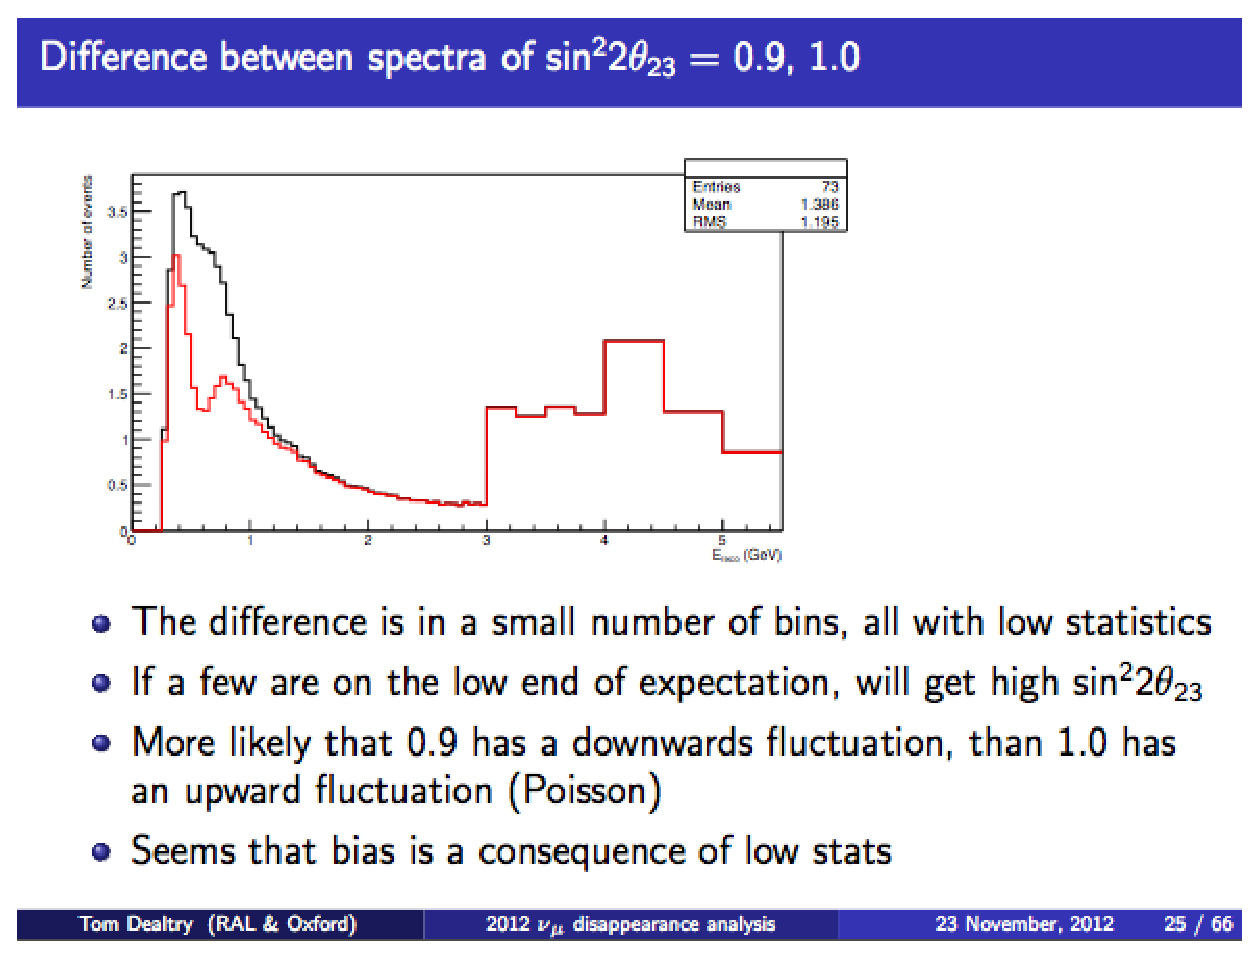
\includegraphics[width=35pc]{./images/slide25_tom_20121123.eps}
\caption {
  Slide 25 in http://www.t2k.org/asg/oagroup/meeting/oameeting20121121/valornumu/view
  (see text for details).
}
\label{fig:slide25}
\end{figure*}

%.......

\begin{figure*}[htb]
\center
\includegraphics[width=35pc]{{./images/28_all_0.900000_skdet_ccnqe_twopulls_rev}.eps}
\caption {
  Plot of $f_{CCnonQE}^{SK}$ pull, using definitions 1 and 2 (see Appendix H in version 2 of T2K-TN-141).
  The plot was generated using the `2+8' fit variant, for true oscillation parameters
  $sin^2(2\theta_{23}) = 0.9$ and $|\Delta m^2_{32}| = 2.4 \times 10^{-3} eV^{2}/c^{4}$.
}
\label{fig:anselmo_q9d}
\end{figure*}

%.......

\begin{figure*}[htb]
\begin{minipage}[t]{0.48\linewidth}
\center
\includegraphics[width=20pc]{{./images/28_all_0.900000_sf_pull_rev}.eps}
\caption {
  Residuals for systematic parameter $f_{SF}$.
  There is a negative bias, as explained in the text, because 
  the nominal value
  of this parameter is at the boundary of its allowed range.
  This is a special case, due to the nature of systematic parameter $f_{SF}$.
  The plot was generated using the `2+8' fit variant, for true oscillation parameters
  $sin^2(2\theta_{23}) = 0.9$ and $|\Delta m^2_{32}| = 2.4 \times 10^{-3} eV^{2}/c^{4}$.
}
\label{fig:anselmo_q9e1}
\end{minipage}
\hspace{0.06\linewidth}
\begin{minipage}[t]{0.48\linewidth}
\center
\includegraphics[width=20pc]{{./images/28_all_0.900000_sf_bestfit_rev}.eps}
\caption {
  Distribution of best-fit values for systematic parameter $f_{SF}$.
  The parameter is limited in the range [0,1] with 0 being the nominal value
  (see T2K-TN-141 for details).
  The plot was generated using the `2+8' fit variant, for true oscillation parameters
  $sin^2(2\theta_{23}) = 0.9$ and $|\Delta m^2_{32}| = 2.4 \times 10^{-3} eV^{2}/c^{4}$.
}
\label{fig:anselmo_q9e2}
\end{minipage}
\end{figure*}


%........................................................................................................
\vspace{5 mm}
\item
{\em
  ``Figs 24-26. It refers  to fig 259. I think it should be 23.''
}\\
\\
Fixed.

%........................................................................................................
\vspace{5 mm}
\item
{\em
  ``In Table 12, how is ndf defined? I guess it should be different for 2+N and 2+8 fits.''
}\\
\\
It is the number of bins minus the number of fit parameters.
There are 73 reconstructed energy bins and 2 oscillation parameters, therefore 71 degrees of freedom.
The nuisance parameters do not contribute.
The inclusion in the fit of nuisance parameters is accompanied by the addition of an equal number
of bins (penalty terms).
We think that both the `2+N' and `2+8' fits have the same number of degrees of freedom.

%........................................................................................................
\vspace{5 mm}
\item
{\em
  ``In line 748 I guess Tab. 17 should be Tab. 12.''
}\\
\\
LateX referencing error fixed.

%........................................................................................................
\vspace{5 mm}
\item
{\em
  ``As mentioned my Neil (I think) it is strange that the the pull values for most systematics are very small. 
    I think at some point you justified that by saying that the fitter is insensitive to them. 
    Even in this case pulls should be gaussianly distributed with sigma close to 1, unless the fit result 
    is biased to the prior for some reason. Probably this is due to the way minuit works. 
    Does minuit use the initial value as fit result in the case the $\chi^2$ of neigbouring points is the same 
    (or very similar) ? If this is the case you should explain it. 
    Anyway, why pull values for the 8 relevant systematic parameters are all below 0.4 while the 
    pull distribution for MC toy experiments is very wide (point 9)?''
}\\
\\
    As you say, the pulls should have a Gaussian distribution with sigma close to 1 \emph{unless the fit result
    is biased to the prior for some reason}. But they are biased to be near the prior value by the penalty 
    term. In the '2+8' fits, 8 systematic parameters are free to move away from their nominal values, while in 
    the '2+N' fits all parameters are free to move. When a systematic parameter that is free to move stays close 
    to its nominal value, this means that the reduction in $\chi^{2}$ in Eq.\ 3 from moving that parameter is 
    less than the corresponding increase in the penalty term. Only certain systematics are able to change the 
    predicted reconstructed energy spectrum to a sufficient extent to offset the penalty term. 

%........................................................................................................
\vspace{5 mm}
\item
{\em
  ``Why don't you merge tables 13 and 12?''
}\\
\\
Done.

%........................................................................................................
\vspace{5 mm}
\item
{\em
  ``Fig. 33 and 34. I guess gof means Goodness-of-fit, this should be defined somewhere in sections 4.2 or 5.2.  
    Where the values $\chi^{2}_{data}$=1, 1.07 come from? 
    I guess this is the result of Eq. 3, isn't it? 
    What is the relation between those numbers and the ones in table 12?''
}\\
\\
In version 2 of T2K-TN-141, The $\chi^{2}_{gof}$ symbol (and `gof') is defined in the caption.
Indeed, $\chi^{2}_{data}$ is obtained from the log-likelihood ratio (Eq.\ 3) and the Run 1+2+3 data, 
using the 5 reconstructed energy bins defined in Sec.\ 4.2.
The $\chi^{2}_{best-fit}$ values are obtained from the same equation and using the same data,
but the data are distributed in the 73 reconstructed energy bins used in the fit.
In version 2, a clarification was added in the caption of Tab.\ 12.
The numbers in Tab.\ 12 are not used for a goodness-of-fit test due to concerns about low statistics in 
some bins, as described in Sec.\ 4.2.

%........................................................................................................
\vspace{5 mm}
\item
{\em
  ``Figs 35, 36 and 37. Why the data points between 2 and 3 GeV in figs 36 and 37 look more significant  
    than the once in fig 35. Those figures are not compatible.
    Same for figs 38-40''
}\\

The errors in the ratio plots are not displayed properly (TH1D::Sumw2() was not called after the
ratios were formed). This will be rectified in version 2 of T2K-TN-141. 

%........................................................................................................
\vspace{5 mm}
\item
{\em
  ``In line 803 you say that the ${\Delta}{\chi}^{2}$ distributions are identical for the 2+N and 2+8 fits. 
    It would say almost identical or very similar.''
}\\
\\
Changed identical to almost identical.

%........................................................................................................
\vspace{5 mm}
\item
{\em
  ``Figs. 47-49 look quite different to 52-54. It took me a while to realize that this is due to the 
    different ranges shown. Would it be possible to have exactly the same range for both fits ? 
    It's a bit misleading''.
}\\
\\
The plots were revised in version 2 of T2K-TN-141. Now, the same range is used for both sets of plots.

%........................................................................................................
\vspace{5 mm}
\item
{\em
  ``Fig 57. referece $\rightarrow$ reference''.
}\\
\\
Fixed.

%........................................................................................................
\vspace{5 mm}
\item
{\em
  ``Figs 61-79. The best fit point is shown in some cases but not always. Is there any reason for that?''
}\\
\\
The plots were revised in version 2 of T2K-TN-141. Now, the best-fit points are shown on all plots.

%........................................................................................................
\vspace{5 mm}
\item
{\em
  ``At line 828 you say again that contours are identical. I would say almost identical.''
}\\
\\
Changed identical to almost identical.

%........................................................................................................
\vspace{5 mm}
\item
{\em
  ``Lines 831-832. What do you mean by the last sentence?''
}\\
\\
The plot to which this sentence refers shows the effect of fitting for 0, 8 and 48 (all) systematic parameters.
Not fitting for any systematics (as was done in the Run1+2 analysis) gives results which are clearly
different from those obtained if we fit for the 8 most important or all 48 systematics.
Therefore, the approach  taken in the Run 1+2 analysis is not applicable in the Run 1+2+3 analysis.
But there is very little difference between the results obtained if we fit for
the 8 most important or all 48 systematics. In view of this similarity between the `2+8' and `2+N'
results, our viewpoint on which one is the preferred result is given in Sec. 5.6.

%........................................................................................................
\vspace{5 mm}
\item
{\em
  ``In section 5.5.2 you show that FC produces wider contours. A comment on that would be probably worth.''
}\\
\\
Typically, with the Feldman and Cousins method, one obtains contours which: 
\begin{itemize}
\item
for maximal mixing, extend over narrower range in $|\Delta m^2_{32}|$, and
\item
in the $|\Delta m^2_{32}|$ range around the best-fit value, extend over wider range
in $sin^{2}(2\theta_{23})$.
\end{itemize}

These features are well understood and they were documented in detail during the Run 1 and Run 1+2 analyses.
It was our intention to add, in version 2 of T2K-TN-141, 
plots of the Run 1+2+3 Feldman and Cousins $\Delta\chi^{2}_{critical}$ surfaces
obtained using the `2+8' and `2+N' 3-flavour fits.
From these surfaces, the features of the  Feldman and Cousins contours are evident.
In any case, an explicit comment will be added as suggested.

%........................................................................................................
\vspace{5 mm}
\item
{\em
  ``Although the it is quite obvious after reading the values for the data it would be better to 
    say explicitly what the dashed lines indicate, either by including them in the 
    legend or by mentioning them in the caption.''
}\\
\\
We think you might be referring to Fig.\ 77. The caption in this figure has been updated in version 2 of 
T2K-TN-141 to better explain the meaning of the dashed lines (the vertical dashed lines show the
minimum excluded value of $sin^{2}(2\theta_{23})$, at 68\% CL and 90\% CL, for the Run 1+2+3 dataset).

%........................................................................................................
\vspace{5 mm}
\item
{\em
  ``There is problem with the colors in Fig. 78. Would it be possible to use the ones in Fig 79 ?''.
}\\
\\
The colour scheme was changed as suggested.

%........................................................................................................
\vspace{5 mm}
\item
{\em
  ``Extra dot after 1.000 at line 906.''
}\\
\\
Fixed.

%........................................................................................................

\end{enumerate}
